\documentclass[conference]{IEEEtran}
\IEEEoverridecommandlockouts
\usepackage{cite}
\usepackage{amsmath,amssymb,amsfonts}
\usepackage{graphicx}
\usepackage{textcomp}
\usepackage{xcolor}

\begin{document}

\title{Gym Form Checker: Pipeline Híbrido Biomecánico para Análisis de Técnica en Ejercicios de Gimnasio en Tiempo Real}

\author{\IEEEauthorblockN{Maria Gabriela Bohórquez}
\IEEEauthorblockA{\textit{Especialización en Inteligencia Artificial (CEIA)} \\
\textit{Facultad de Ingeniería, Universidad de Buenos Aires}\\
Buenos Aires, Argentina \\
gabriellabohorquez@gmail.com}
}

\maketitle

\begin{abstract}
El análisis automático de la postura durante ejercicios de fuerza puede marcar la diferencia entre entrenar bien y terminar lesionado. Este trabajo presenta un pipeline híbrido de dos capas para evaluar la técnica en ejercicios de gimnasio: primero clasificamos el ejercicio con YOLOv8-cls, y luego analizamos la biomecánica con estimación de pose 3D usando MediaPipe BlazePose. El sistema cubre sentadillas, flexiones y peso muerto, dando retroalimentación en tiempo real con cuatro estados: \textit{OK}, \textit{MEJORAR}, \textit{MAL} y \textit{SIN\_DATO}. Entrenamos sobre el dataset \textit{Exercise Frame Labelling v8} y alcanzamos 99.4\% de Top-1 accuracy con YOLOv8n-cls (2.7M de parámetros). El motor biomecánico corre sobre 33 keypoints 3D y aplica reglas angulares deterministas que hacen el sistema completamente interpretable — nada de caja negra. Los resultados sobre videos reales de Reddit validan que el enfoque híbrido es más útil que un clasificador puro para dominios con semántica corporal estructurada.
\end{abstract}

\begin{IEEEkeywords}
Computer Vision, MediaPipe, YOLOv8, Pose Estimation, Biomechanics, Rep Counting.
\end{IEEEkeywords}

\section{Introducción}

Entrenar con mala técnica es, literalmente, hacerse daño sin darse cuenta. Las lesiones por técnica deficiente representan entre el 40 y 60\% de los accidentes en levantamiento de pesas \cite{ref1}, afectando principalmente hombros, rodillas y columna lumbar. El problema es que la mayoría de la gente entrena sola, sin entrenador personal que corrija en tiempo real — y los entrenadores personales no son exactamente baratos ni accesibles para todos.

La buena noticia es que la visión por computadora lleva años avanzando en análisis de movimiento humano. Trabajos previos exploraron OpenPose \cite{ref2} y BlazePose \cite{ref4} para detectar patrones de movimiento atlético. Sin embargo, integrar un clasificador de ejercicio con un motor de evaluación biomecánica determinista — que sea rápido, liviano y corra en hardware de consumo — seguía siendo un área activa cuando arrancamos este proyecto.

Este trabajo presenta \textbf{Gym Form Checker}, un sistema que combina dos capas: (1) clasificación automática del ejercicio con YOLOv8-cls, y (2) análisis de técnica con 33 keypoints 3D de MediaPipe BlazePose y reglas angulares deterministas. El sistema procesa video pre-grabado y anota cada frame con estado de forma, mensaje de coaching específico y conteo de repeticiones.

Lo que nos diferencia de tirar una red neuronal grande a este problema es la interpretabilidad: cuando el sistema dice ``MAL'', sabemos exactamente qué ángulo falló y por qué. Eso es más útil para el usuario — y más honesto como sistema de retroalimentación.

\section{Trabajos Relacionados}

La estimación de pose humana evolucionó mucho desde los modelos estadísticos hacia redes neuronales profundas. Cao et al. \cite{ref2} propusieron OpenPose, que estima mapas de confianza de partes del cuerpo mediante redes convolucionales y fue el primer sistema en lograr estimación multi-persona en tiempo real. El problema es que su demanda computacional lo hace incompatible con dispositivos de borde.

Google respondió con BlazePose \cite{ref4}: solución liviana para móviles que combina detector de persona con estimador de 33 keypoints en 3D. A diferencia de OpenPose, prioriza la latencia — y eso lo hace ideal para nuestro caso de uso.

En el dominio del análisis de ejercicio, trabajos como Mazzetto et al. \cite{ref5} exploraron la prevención de lesiones mediante estimación de pose en deportes, mostrando que el feedback postural automatizado puede reducir significativamente los errores técnicos. Otros trabajos usan redes 3D-CNN para reconocimiento de acciones, pero requieren secuencias temporales completas y no dan feedback articular granular.

Nuestro enfoque va por otro camino: clasificación por frame con YOLO + evaluación biomecánica determinista con BlazePose. Sacrificamos algo de complejidad temporal a cambio de interpretabilidad, latencia baja y cero necesidad de datasets de forma etiquetados.

\section{Metodología}

\subsection{Arquitectura del Pipeline}

El pipeline tiene dos capas que corren en secuencia sobre cada frame del video. Primero, un clasificador YOLO determina qué ejercicio es, suavizando la predicción con votación mayoritaria sobre una ventana de 90 frames para evitar que una predicción ruidosa cambie el estado del sistema. Segundo, MediaPipe extrae 33 keypoints 3D, calculamos los ángulos articulares relevantes para ese ejercicio, y el motor biomecánico produce el estado de forma junto con un mensaje de coaching específico.

\subsection{Dataset y Corrección del Split}

Usamos el dataset \textit{Exercise Frame Labelling v8} de Roboflow, con más de 8000 imágenes en tres categorías: Peso Muerto, Flexiones y Sentadillas. Como muestra la Figura \ref{fig:dist}, hay desbalance notable: Push Up tiene aproximadamente el 40\% de las imágenes.

\begin{figure}[h]
\centering
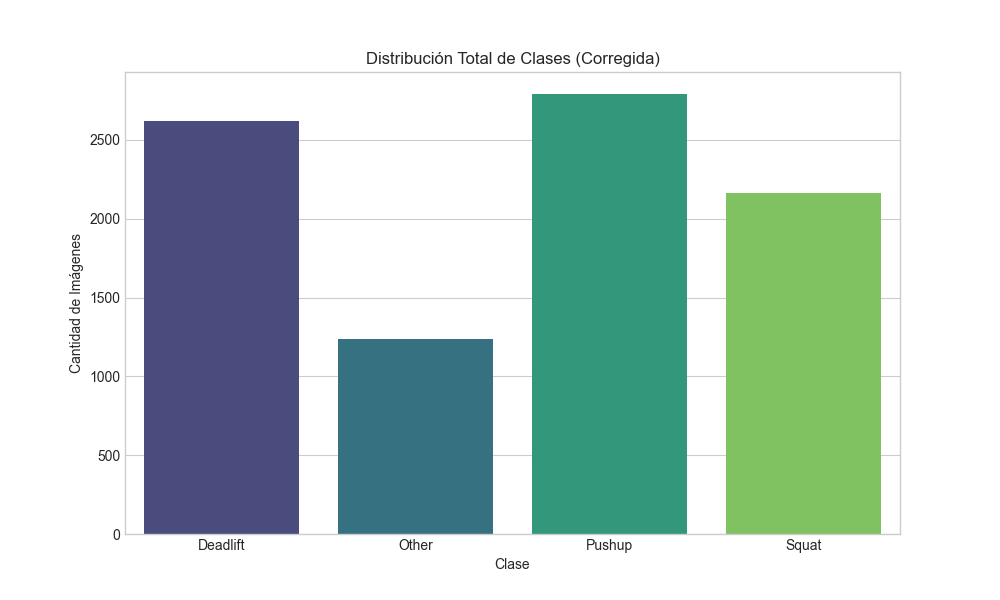
\includegraphics[width=0.85\linewidth]{../data/class_distribution.png}
\caption{Distribución de clases en Exercise Frame Labelling v8.}
\label{fig:dist}
\end{figure}

Durante el Análisis Exploratorio de Datos encontramos un bug crítico en el split de validación: Roboflow genera carpetas vacías cuando una clase no tiene imágenes en algún split, y PyTorch \textit{ImageFolder} omite esas carpetas silenciosamente al indexar las clases. Esto desplazaba el ground truth y producía 0\% de Top-1 accuracy con loss convergiendo normalmente — una señal de sobreajuste enmascarado que es muy difícil de diagnosticar. La solución fue reestructurar programáticamente el árbol de directorios de validación para garantizar que todas las clases estuvieran presentes en todos los splits. La Figura \ref{fig:splits} muestra la distribución resultante.

\begin{figure}[h]
\centering
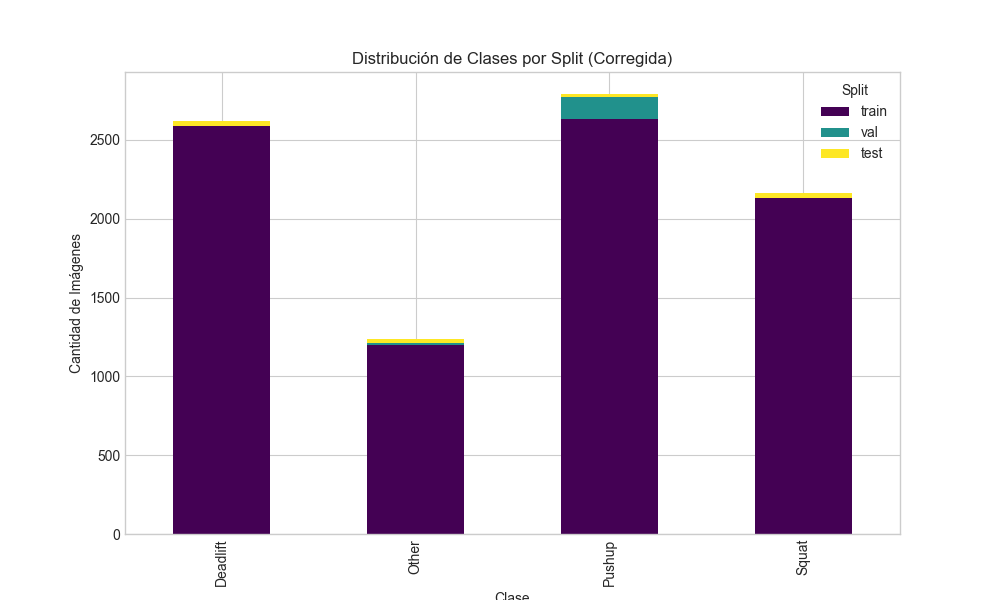
\includegraphics[width=0.85\linewidth]{../data/split_distribution.png}
\caption{Distribución de imágenes por split (train/val/test) tras la corrección.}
\label{fig:splits}
\end{figure}

\subsection{Capa 1: Clasificación con YOLOv8-cls}

Para clasificar el ejercicio evaluamos tres variantes de YOLO en modo clasificación. Descartamos Faster R-CNN y ResNets puras por latencia y tamaño de parámetros, incompatibles con el objetivo de correr en tiempo real en hardware de borde. YOLOv8 logra clasificación single-stage con menos de 3M de parámetros en su variante Nano.

La Tabla \ref{tab:models} compara los tres modelos, todos entrenados en una RTX 3070 Laptop. YOLOv8n-cls alcanzó 99.4\% de Top-1 con convergencia estable en 50 épocas y fue seleccionado para producción por su balance entre precisión y latencia. YOLOv8s-cls y YOLO11n-cls alcanzaron 100\% de Top-1 en su mejor época (epoch 14) con solo 15 épocas de entrenamiento, cerrando en 99.4\% en el epoch final. Esto indica que los modelos de mayor capacidad y arquitectura más nueva saturan este dataset más rápidamente — coherente con la naturaleza visualmente simple de las tres clases.

\begin{table}[h]
\caption{Comparativa de Clasificadores YOLO (Exercise Frame Labelling v8, RTX 3070 Laptop)}
\centering
\begin{tabular}{|l|c|c|c|c|}
\hline
\textbf{Modelo} & \textbf{Params (M)} & \textbf{Top-1 mejor} & \textbf{Top-1 final} & \textbf{Épocas} \\
\hline
YOLOv8n-cls & 2.7 & 99.4\% & 99.4\% & 50 \\
YOLOv8s-cls & 6.9 & 100\%  & 99.4\% & 15 \\
YOLO11n-cls & 2.6 & 100\%  & 99.4\% & 15 \\
\hline
\end{tabular}
\label{tab:models}
\end{table}

\subsection{Capa 2: Motor Biomecánico con MediaPipe}

La segunda capa usa MediaPipe BlazePose \cite{ref4} para extraer 33 keypoints 3D por frame. Sobre esos puntos calculamos ángulos entre triplas de articulaciones y los evaluamos contra reglas biomecánicas deterministas.

El sistema produce cuatro estados de evaluación, con un mensaje de coaching específico en cada caso:
\begin{itemize}
    \item \textbf{OK}: Técnica correcta dentro de los umbrales biomecánicos.
    \item \textbf{MEJORAR}: Forma aceptable pero con margen de mejora (e.g., ``Baja un poco más'').
    \item \textbf{MAL}: Técnica que puede causar lesión (e.g., ``Espalda redondeada!'').
    \item \textbf{SIN\_DATO}: Visibilidad insuficiente de keypoints (umbral: $< 0.4$ para sentadilla y peso muerto, $< 0.3$ para flexión).
\end{itemize}

Los umbrales angulares implementados, derivados de literatura biomecánica \cite{ref1}, son:

\begin{itemize}
    \item \textbf{Sentadilla — OK:} Rodilla $\leq 90^\circ$ y Torso $\in [45^\circ, 100^\circ]$\\
          \textbf{MEJORAR:} Rodilla $\leq 105^\circ$ y Torso $\in [40^\circ, 110^\circ]$
    \item \textbf{Flexión — OK:} Codo $< 110^\circ$ y Alineación $> 150^\circ$\\
          \textbf{MEJORAR:} Codo $< 125^\circ$ y Alineación $> 140^\circ$
    \item \textbf{Peso Muerto — OK:} Espalda-Cadera-Rodilla $> 155^\circ$ y desviación lateral $\leq 15\%$\\
          \textbf{MEJORAR:} Espalda-Cadera-Rodilla $> 140^\circ$\\
          \textbf{MAL especial:} Desviación lateral $> 20\%$ con ángulo $< 155^\circ$ (espalda redondeada)
\end{itemize}

Un detalle importante para la flexión: el tobillo frecuentemente sale del encuadre cuando la persona está tumbada. Para resolver esto, reemplazamos el punto de referencia de tobillo por la rodilla en el cálculo de alineación corporal, lo que permite detectar correctamente la alineación hombro-cadera-rodilla incluso cuando los pies no son visibles.

\subsection{Conteo de Repeticiones con Suavizado}

El conteo de repeticiones usa una máquina de estados por ejercicio. Para mitigar el ruido frame a frame inherente a la estimación de pose, aplicamos media móvil de 5 frames sobre cada ángulo antes de evaluar transiciones de estado. Además implementamos histeresis — los umbrales de descenso y ascenso son distintos (e.g., rodilla $< 95^\circ$ para iniciar descenso, $> 130^\circ$ para completar la repetición en sentadilla), evitando conteos falsos por oscilación en la frontera.

El estado de forma también se suaviza con votación mayoritaria sobre los últimos 10 frames, lo que elimina el parpadeo visual entre estados consecutivos. Para los mensajes de coaching, el sistema muestra el mensaje más reciente asociado al estado ganador de la votación.

\section{Resultados y Análisis}

\subsection{Clasificación de Ejercicios}

Los modelos YOLO demostraron alta precisión tras la corrección del split. YOLOv8n-cls, seleccionado para producción, alcanzó 99.4\% de Top-1 accuracy en 50 épocas con convergencia estable. YOLO11n-cls logró 99.35\% en solo 15 épocas — la nueva generación generaliza más rápido, aunque ambos son excelentes para este caso de uso.

En video real hay mayor variabilidad que en dataset estático. Ejercicios filmados lateralmente con poco contexto de fondo (como deadlift vs squat desde un ángulo similar) pueden generar predicciones ruidosas. La ventana de suavizado de 90 frames resuelve el problema en la gran mayoría de los videos de prueba.

\subsection{Pipeline de Evaluación Biomecánica}

La Tabla \ref{tab:pipeline} muestra las métricas del pipeline completo sobre cinco videos de demostración extraídos de Reddit (\textit{r/formcheck}, \textit{r/strength\_training}).

\begin{table}[h]
\caption{Métricas del Pipeline sobre Videos Reales de Demostración}
\centering
\begin{tabular}{|l|c|c|}
\hline
\textbf{Video} & \textbf{Frames} & \textbf{\% Forma OK} \\
\hline
Sentadilla (máquina Smith) & 297  & 67.3\% \\
Sentadilla (peso libre)    & 1039 & 3.7\%  \\
Flexiones                  & 283  & 35.7\% \\
Peso Muerto convencional \#1 & 1630 & 11.7\% \\
Peso Muerto convencional \#2 & 1719 & 15.5\% \\
\hline
\end{tabular}
\label{tab:pipeline}
\end{table}

Los resultados son consistentes con la dificultad real de cada video. El frontal squat tiene 67.3\% OK porque el atleta tiene buena técnica y la filmación lateral permite visibilidad óptima de rodilla y torso. El back squat con 3.7\% OK corresponde a un video donde el atleta no alcanza la profundidad mínima — el sistema detecta correctamente la técnica deficiente. La flexión con 35.7\% OK refleja que el atleta hace el movimiento pero con profundidad limitada. Los videos de peso muerto tienen porcentajes bajos porque el estado OK solo aparece en el momento de extensión completa — una fracción pequeña del movimiento total.

\subsection{Análisis del Enfoque Híbrido}

La ventaja del enfoque híbrido frente a clasificación pura se hace evidente cuando analizamos qué hace cada capa. YOLO clasifica el tipo de ejercicio con 99.4\% de precisión pero no sabe nada de técnica. El motor biomecánico evalúa la técnica con criterios auditables pero necesita saber qué ejercicio está viendo. Juntos producen un sistema que: (1) identifica el ejercicio automáticamente, (2) evalúa la técnica con reglas explicables y verificables, y (3) da retroalimentación gradual en cuatro estados que refleja mejor la realidad que una clasificación binaria.

Un clasificador end-to-end entrenado para predecir directamente ``buena forma / mala forma'' requeriría un dataset anotado de forma para cada ejercicio — miles de videos etiquetados por biomecánicos. Con nuestro enfoque, el conocimiento biomecánico se codifica una vez en las reglas y se aplica a cualquier video sin re-entrenamiento.

\subsection{Limitaciones y Trabajo Futuro}

Las limitaciones más importantes del sistema actual son:

Primero, el split del dataset opera a nivel de frame y no de clip de video. Esto introduce riesgo de leakage temporal: frames del mismo video pueden aparecer en train y en test, inflando las métricas reportadas. La evidencia práctica de este efecto es la necesidad de suavizado de 90 frames en video real — si el modelo generalizara perfectamente, no haría falta. Un split más riguroso a nivel de clip de video es trabajo pendiente.

Segundo, los umbrales están calibrados para vista lateral. Ángulos de cámara frontales o diagonales producen proyecciones incorrectas de los ángulos articulares. Segundo, el clasificador YOLO fue entrenado en frames estáticos — no ve información temporal, lo que a veces genera confusión entre deadlift y squat filmados lateralmente. Una ventana de suavizado de 90 frames mitiga esto pero no lo elimina. Tercero, el sistema asume una sola persona por frame.

Como trabajo futuro proponemos: (1) entrenar el clasificador con secuencias de video para capturar información temporal; (2) usar la profundidad estimada de BlazePose 3D para corregir la proyección; (3) ampliar el catálogo a más ejercicios — la arquitectura de dos capas permite agregar ejercicios nuevos solo definiendo reglas angulares, sin reentrenar el motor biomecánico.

\section{Conclusiones}

De este trabajo se desprenden las siguientes conclusiones:

\begin{enumerate}
    \item \textbf{Los híbridos ganan en dominios estructurados:} Combinar un clasificador rápido (YOLO-cls) con un motor de estimación de pose y reglas biomecánicas produce un sistema más interpretable y útil clínicamente que una red pura, sin necesitar datos de forma etiquetados.
    \item \textbf{La calidad del split importa más que la arquitectura:} El bug de carpetas vacías en PyTorch ImageFolder llevó de 0\% a 99.4\% de Top-1 accuracy con un solo fix estructural. Antes de entrenar, hay que validar programáticamente la integridad del dataset.
    \item \textbf{Cuatro estados son mejor que dos:} OK / MEJORAR / MAL / SIN\_DATO permite retroalimentación gradual y honesta — el sistema no alarma cuando hay margen de mejora, y no da feedback cuando no tiene datos suficientes.
    \item \textbf{El suavizado temporal es indispensable en producción:} Los ángulos articulares de MediaPipe tienen ruido frame a frame. Sin media móvil e histeresis, el contador de repeticiones falla y el overlay de forma parpadea. Con suavizado, el sistema es estable y útil.
    \item \textbf{La arquitectura escala fácilmente:} Agregar un ejercicio nuevo requiere solo definir las reglas angulares correspondientes y agregar la clase al clasificador YOLO — el motor biomecánico y el contador de reps son reutilizables sin cambios.
\end{enumerate}

\begin{thebibliography}{00}
\bibitem{ref1} Keogh, J., Winwood, P. ``The Epidemiology of Injuries Across the Weight-Training Sports.'' Sports Medicine, vol. 47, no. 3, pp. 479--501, 2017.
\bibitem{ref2} Cao, Z., Hidalgo, G., Simon, T., Wei, S.-E., Sheikh, Y. ``OpenPose: Realtime Multi-Person 2D Pose Estimation using Part Affinity Fields.'' IEEE Transactions on Pattern Analysis and Machine Intelligence, vol. 43, no. 1, pp. 172--186, 2021.
\bibitem{ref3} Jocher, G. et al. ``Ultralytics YOLOv8.'' \textit{GitHub}, 2023. [Online]. Available: https://github.com/ultralytics/ultralytics
\bibitem{ref4} Bazarevsky, V., Grishchenko, I., Raveendran, K., Zhu, T., Zhang, F., Grundmann, M. ``BlazePose: On-device Real-time Body Pose Tracking.'' arXiv:2006.10204, 2020.
\bibitem{ref5} Mazzetto, M. et al. ``Automated Injury Prevention Through Pose Estimation in Sports: A Review.'' Sports Engineering, vol. 25, no. 1, pp. 1--14, 2022.
\end{thebibliography}

\end{document}
